\documentclass{beamer}
\usefonttheme[onlymath]{serif}

\title{A Gentle Introduct to TensorFlow}
\author{Rebecca Skinner}
\institute{Asteris}
\date{\today}
\mode<presentation> {\usetheme{Madrid}}

\usepackage[english]{babel}
\usepackage[latin1]{inputenc}
\usepackage{times}
\usepackage[T1]{fontenc}
\usepackage{hyperref}
\usepackage{listings}
\usepackage{color}
\usepackage{amsmath}
\usepackage{csquotes}
\usepackage{verbatim}
\usepackage{animate}

% \usecolortheme[RGB={221,211,255}]{structure}

\definecolor{comment}{rgb}{145,175,188}
\definecolor{keyword}{rgb}{157,163,199}
\definecolor{string}{rgb}{155,204,174}

\lstset{
  backgroundcolor=\color{white},
  basicstyle=\tiny,
  keywordstyle=\color{keyword},
  commentstyle=\color{comment},
  showspaces=false,
  showstringspaces=false,
  showtabs=false,
  stringstyle=\color{string},
  tabsize=4
}

\newcommand{\chref}[3] {
  {\color{#1} \href{#2}{\underline{#3}}}
}

\AtBeginSection[]{
  \begin{frame}
  \vfill
  \centering
  \begin{beamercolorbox}[sep=8pt,center,shadow=true,rounded=true]{title}
    \usebeamerfont{title}\insertsectionnumber \\ \insertsectionhead\par%
  \end{beamercolorbox}
  \vfill
  \end{frame}
}

\AtBeginSubsection[]{
  \begin{frame}
  \vfill
  \centering
  \begin{beamercolorbox}[sep=8pt,center,shadow=true,rounded=true]{title}
    \usebeamerfont{title}\insertsectionnumber.\insertsubsectionnumber\\\insertsubsectionhead\par%
  \end{beamercolorbox}
  \vfill
  \end{frame}
}

\begin{document}

\begin{frame}
  \titlepage{}
\end{frame}

\section{Introduction}

\begin{frame}
  \frametitle{Questions}

  Please feel free to ask questions during this talk by raising your hand.

  {\bf Remember}: If you have a question others were probably wondering the same thing!
\end{frame}


\begin{frame}
  \frametitle{Background}
  % I want to talk a little bit about my background and why I decided
  % to start learning tensorflow- and why I wanted to start talking
  % about it.  One of my key areas of interest is in working with
  % computer vision.  I've also spent a lot of time working in the
  % security field and have been getting more and more interested in
  % applying machine learning techniques to network security analysis.
  I'm a developer with no particular background in Machine Learning or
  Data Science.  So what got me interested in TensorFlow?
  \begin{itemize}
    \item Image Processing
    \item Great Documentation
    \item Language Bindings (C++, Go, Haskell)
  \end{itemize}
\end{frame}

\begin{frame}
  \frametitle{Goals}
  Demistify the language and concepts around TensorFlow so that you
  can start learning it in confidence.
\end{frame}

\begin{frame}
  \frametitle{In This Talk}

  \begin{itemize}
  \item What Is TensorFlow?
  \item When is TensorFlow Useful?
  \item Examples
  \item Final Questions
  \end{itemize}
\end{frame}


\section{What Is Tensorflow?}

\begin{frame}
  \frametitle{What is TensorFlow?}

  {\it TensorFlow lets you perform linear transformations on tensors
    using stateful data flow graphs.}\\
  \vfill
  Whew! that's a lot of words!  This section will
  go into the definitions of some of these words then we'll put those
  definitions all back together.
\end{frame}

\subsection{Tensors}

\begin{frame}[fragile]
  \frametitle{What are Tensors?}

  TensorFlow uses the idea of multidimensional arrays as tensors,
  although the analogy to pure mathematical tensors breaks down under
  scrutiny we'll handwave over the differences right now for the sake
  of clarity.  So what is are tensors?  First let's look at Scalars
  and Vectors.

\end{frame}

\begin{frame}
  \frametitle{Scalars and Vectors}

  Tensors generalize the idea of vectors.  What does that mean? Let's
  look at some examples of Scalar and Vector values.
  \begin{itemize}
  \item {\it scalar}: A scalar is a single value.  It has no
    dimensionality, meaning it's {\it rank 0}.
    \begin{itemize}
    \item $7$
    \item $x$
    \end{itemize}
  \item {\it vector}: A vector has a magnitude and direction.  It can
    be expressed as an array of values. It has a single dimension, so
    it's {\it rank 1}.
    \begin{itemize}
    \item $[1,2]$
    \item $[x,\sigma,\varphi]$
    \end{itemize}
  \end{itemize}
\end{frame}

\begin{frame}[fragile]
  \frametitle{Tensors}

  Tensors can be thought of like a scalar or vector but with
  potentially more dimensions.  Let's look at a {\it rank 2} tensor:
  \[
    \begin{bmatrix}
      x_{0,0} & x_{0,1} & x_{0,2} \\
      x_{1,0} & x_{1,1} & x_{1,2} \\
      x_{2,0} & x_{2,1} & x_{2,2}
    \end{bmatrix}
  \]
\end{frame}

\begin{frame}
  \frametitle{Visualizing Tensor Rank}

  Let's visualize how tensors of rank 1, 2, and 3 look together:
  \begin{figure}
    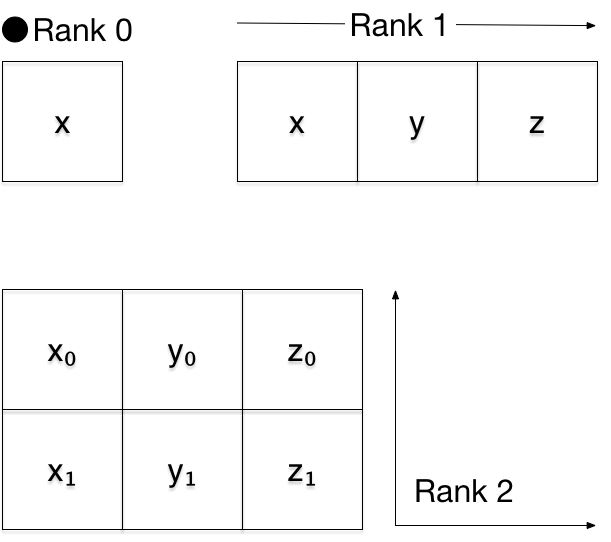
\includegraphics[scale=0.3]{img/tensor_ranks}
    \caption{Visualizing Tensor Ranks}
  \end{figure}
\end{frame}

\begin{frame}
  \frametitle{Structure}

  When we talk about tensors and rank it's useful to think about
  \emph{structure}.  We'll use the term a little loosely in this
  presentation.

  Structures are properties associated with a set.  When we're talking
  about the structure of a tensor we are talking about things like:

  \begin{itemize}
  \item It's ordering
  \item It's dimensions or rank
  \item It's geometry or toplogy
  \end{itemize}

  Structure-preserving operations are called \emph{mappings} or
  \emph{homomorphisms}.  They are operations that preserve the
  structure of the tensor.  Other operations are
  non-structure-preserving.
\end{frame}


\subsection{Linear Transformations}

\begin{frame}
  \frametitle{Linear Transformations}

  \emph{Linear transformation} is a fancy name for the operations we
  can do on our tensors.  In TensorFlow these are the functions that
  we define that operate on our input and provide some output.

  When we look at data flow graphs keep in mind that each of our
  operations are actually linear transformations.
\end{frame}

\begin{frame}
  \frametitle{Linear Transformation Metadata}

  Tensorflow allows for additional information to be attached to
  linear transformations.  This additional information helps fine-tune
  and control the execution of the data flow graph.

  Metadata can include information such as:
  \begin{itemize}
    \item What value types is the transformation compatable with?
    \item What dimiensionality is supported by the transformation?
    \item How many inputs and outputs does it have?
  \end{itemize}
\end{frame}

\subsection{Data Flow Graphs}

\begin{frame}
  \frametitle{What's a Data Flow Graph?}

  DFGs (Data Flow Graphs) are a way of representing operations as
  directed graphs.  Each node in the graph represents a function; and
  the direction of the edges represent the flow of data through the
  system.
\end{frame}

\begin{frame}
  \frametitle{Visualizing Flow Graphs}

  Let's look at a couple of examples of basic arithmetic encoded into
  a DFG.  These could also be other linear relations as well, but
  we'll stick to scalar arithmetic for simplicity.
\end{frame}


\begin{frame}
  \frametitle{Example 1}

  This DFG shows simple addition.  The $a$ and $b$ nodes take no
  inputs and output a value.  The $+$ node takes two inputs and
  returns their sum.
  \begin{figure}
    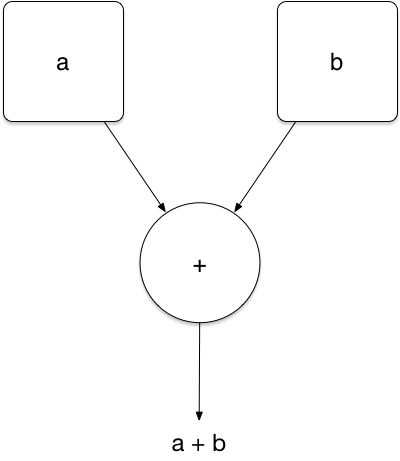
\includegraphics[scale=0.3]{img/a_plus_b}
    \caption{Data Flow Graph for $a + b$}
  \end{figure}
\end{frame}

\begin{frame}
  \frametitle{Example 2}

  Here we Show how we take the result of $a + b$ and pass it back into
  $+$ along with $c$ to get $a + b + c$
  \begin{figure}
    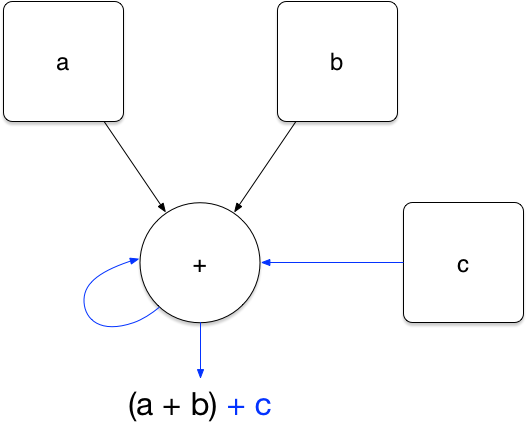
\includegraphics[scale=0.3]{img/a_plus_b_plus_c}
    \caption{Data Flow Graph for $a + b + c$}
  \end{figure}
\end{frame}


\begin{frame}
  \frametitle{Example 3}

  Here we can perform $a * b$ and $x * y$ in parallel.  The outputs,
  $ab$ and $xy$ are passed into $+$ giving $ab + xy$
  \begin{figure}
    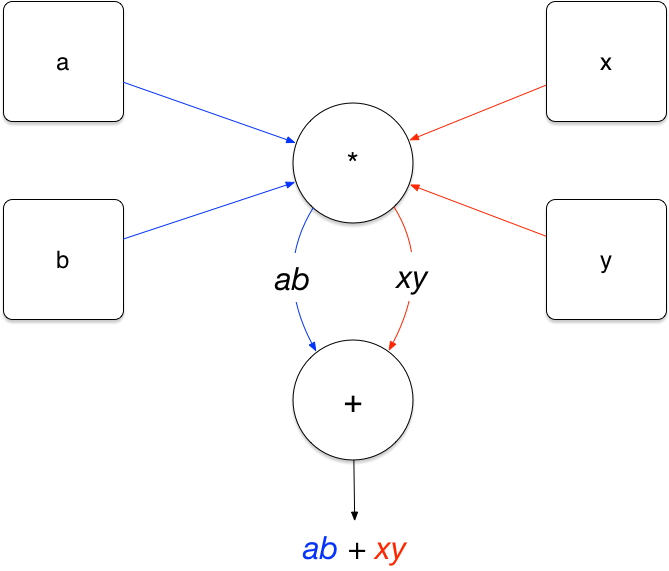
\includegraphics[scale=0.25]{img/ab_plus_xy}
    \caption{Data Flow Graph for $ab + xy$}
  \end{figure}
\end{frame}

\subsection{Putting It All Together}

\begin{frame}
  \frametitle{Let's Put These Concepts Together}

  Now that we understand what a DFG, a Tensor, and a Linear
  Transformation are, let's take a look back at how everything fits
  together.  In the next slide we'll show some code and how the DFG
  will look at a conceptual level.
\end{frame}

\begin{frame}[fragile]
  \frametitle{Sample Code}

  \begin{figure}[fragile]
    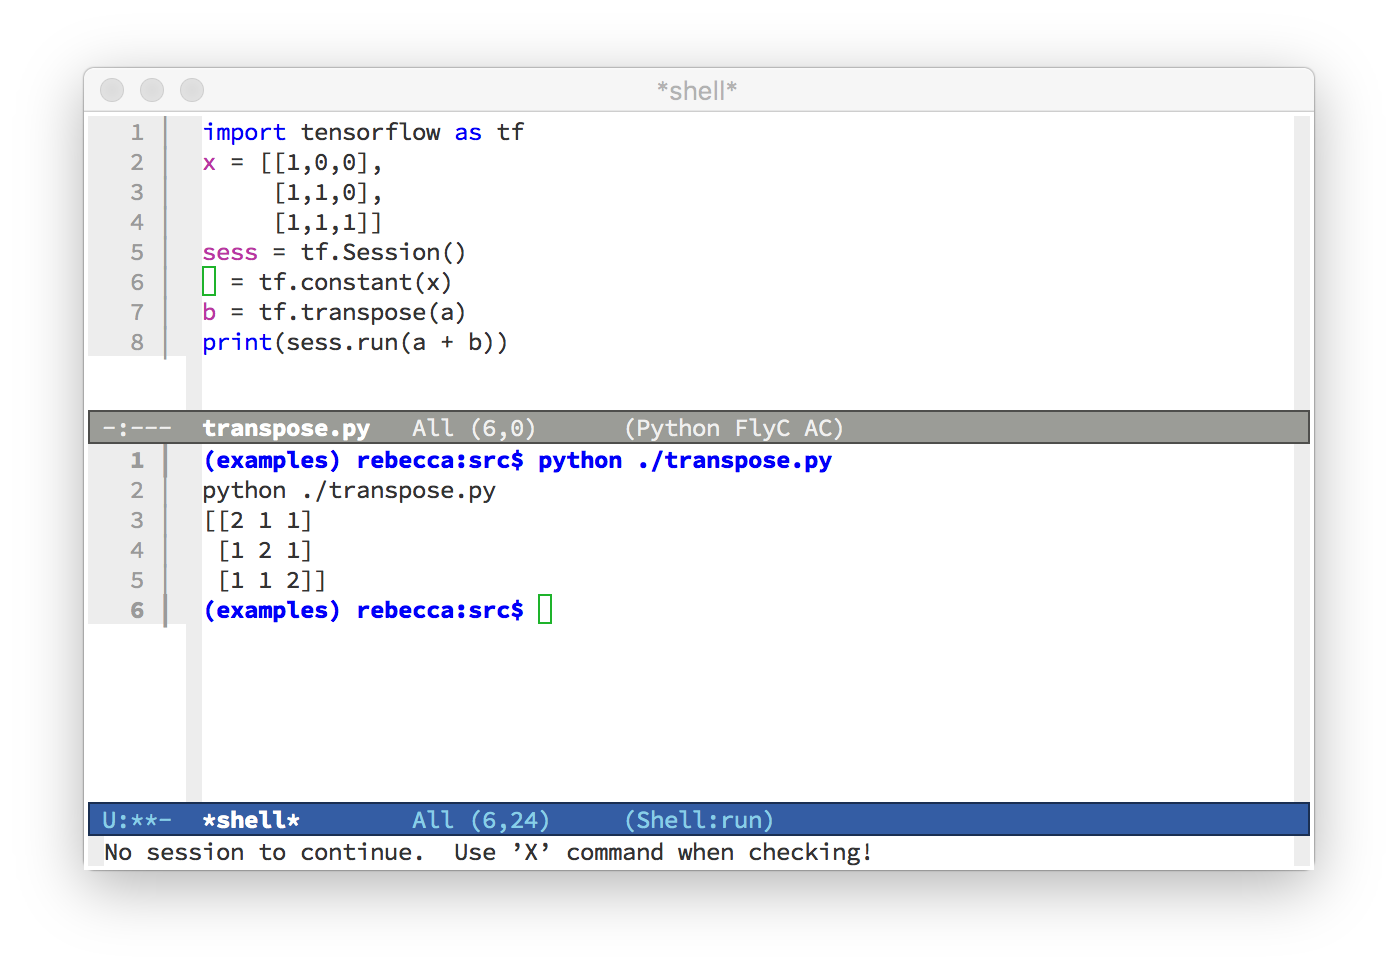
\includegraphics[scale=.4]{img/transpose}
    \caption{Calulating the sum of a matrix and it's transposition}
  \end{figure}
\end{frame}

\begin{frame}[fragile]
  \frametitle{Sample DFG}

  \begin{figure}[fragile]
    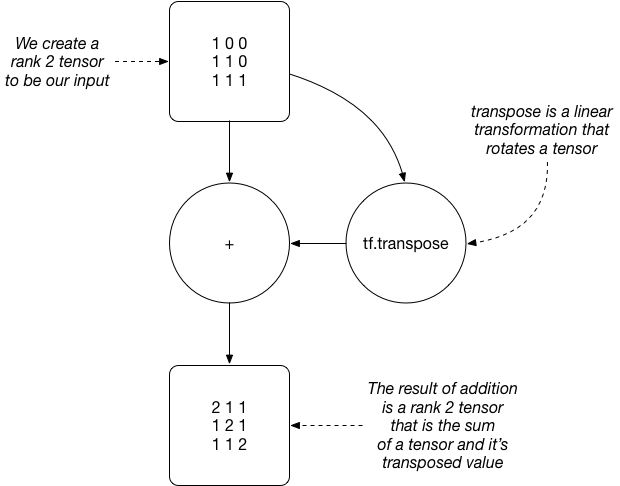
\includegraphics[scale=.3]{img/full_dfg}
    \caption{Visualization of our sample code}
  \end{figure}
\end{frame}

\section{When Can We Use TensorFlow?}

\begin{frame}
  \frametitle{What's Built-In}

  TensorFlow is intended for machine learning tasks, and comes with
  tools built in for performing machine learning against visual and
  linguistic data.  It works best when:

  \begin{itemize}
  \item Data can be represented as a tensor
  \item Operations can be represented as linear transformations
  \item Transformations can happen in parallel or with partial data
  \end{itemize}
\end{frame}

\begin{frame}
  \frametitle{Creating Tensors}

  How can we translate our information into a format that we can use
  with TensorFlow?  Let's look at image data as an example.
\end{frame}

\begin{frame}
  \frametitle{Grayscale Images}

  \begin{figure}
    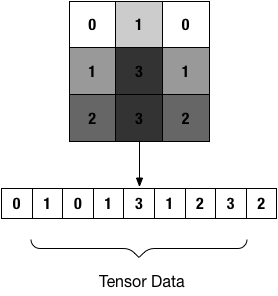
\includegraphics[scale=.65]{img/tensor_basic}
    \caption{3x3 image with 2-bit colorspace serialized to a rank-1 tensor}
  \end{figure}
\end{frame}

\begin{frame}
  \frametitle{Tensor-ifying Images}

  Making our data useful with tensorflow requires thinking about how
  much structure we want to preserve.  In many cases we can give up
  structure to reduce the complexity of our data.  Here are some
  things we've done with our image to reduce it's complexity:
  \begin{columns}
    \begin{column}{0.5\textwidth}
      \begin{itemize}
      \item remove structure by converting it from 2D to 1D
      \item reduce the color space from 24bit to 2bit
      \item reduce the size of the image by lowing it's resolution
      \end{itemize}
    \end{column}
    \begin{column}{0.5\textwidth}
        \begin{figure}
          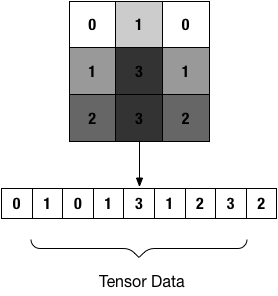
\includegraphics[scale=.25]{img/tensor_basic}
        \end{figure}
    \end{column}
  \end{columns}
\end{frame}

\subsection{Going Beyond Images}

\begin{frame}
  \frametitle{Working with other kinds of data}

  TensorFlow has first-class support for image and lingustic data, but
  it can be used for any type of data where the tensor flowgraph model
  is appropriate.

  Let's talk about some other examples of data we could look at:

  \begin{itemize}
  \item Voice Recordings
  \item Network Traffic
  \item Facial Recognition Data
  \end{itemize}
\end{frame}

\begin{frame}
  \frametitle{Visualizing Tensor Data}

  When we're working with non-visual data, having a visual model for
  how our data is being represented as tensors is helpful. Let's look
  at how we can take a few rank-1 tensors and visualize them as points
  in a 2-D space.

  \begin{figure}
    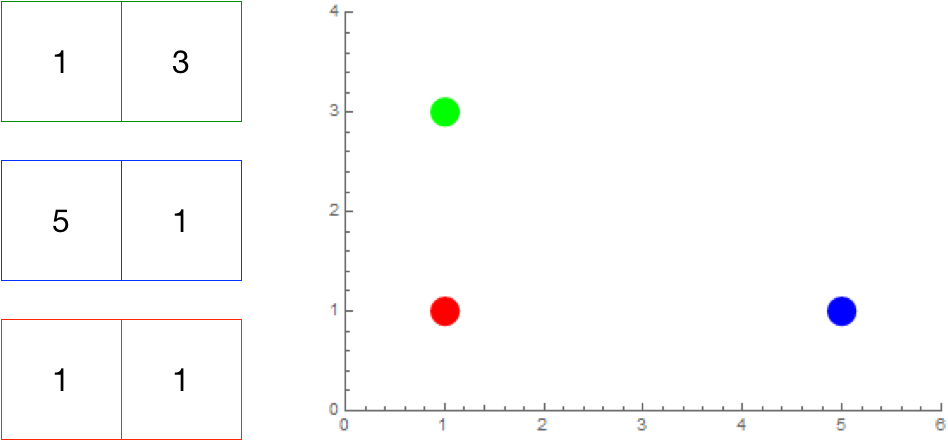
\includegraphics[scale=.2]{img/tensor_2d_graph}
    \caption{Points in 2D space are defined by rank-1 tensors of size 2}
  \end{figure}
\end{frame}

\section{Example: Image Convolution}

\begin{frame}
  \frametitle{Attribution}

  This example is adapted from: ``\emph{Playing with convolutions in TensorFlow}''
  \begin{itemize}
    \item \url{http://mourafiq.com/2016/08/10/playing-with-convolutions-in-tensorflow.htm}
    \item \url{https://github.com/mouradmourafiq/tensorflow-convolution-models}
  \end{itemize}
\end{frame}

\begin{frame}
  \frametitle{Gaussian Blur}
  \begin{columns}
    \begin{column}{0.5\textwidth}
      \begin{figure}
        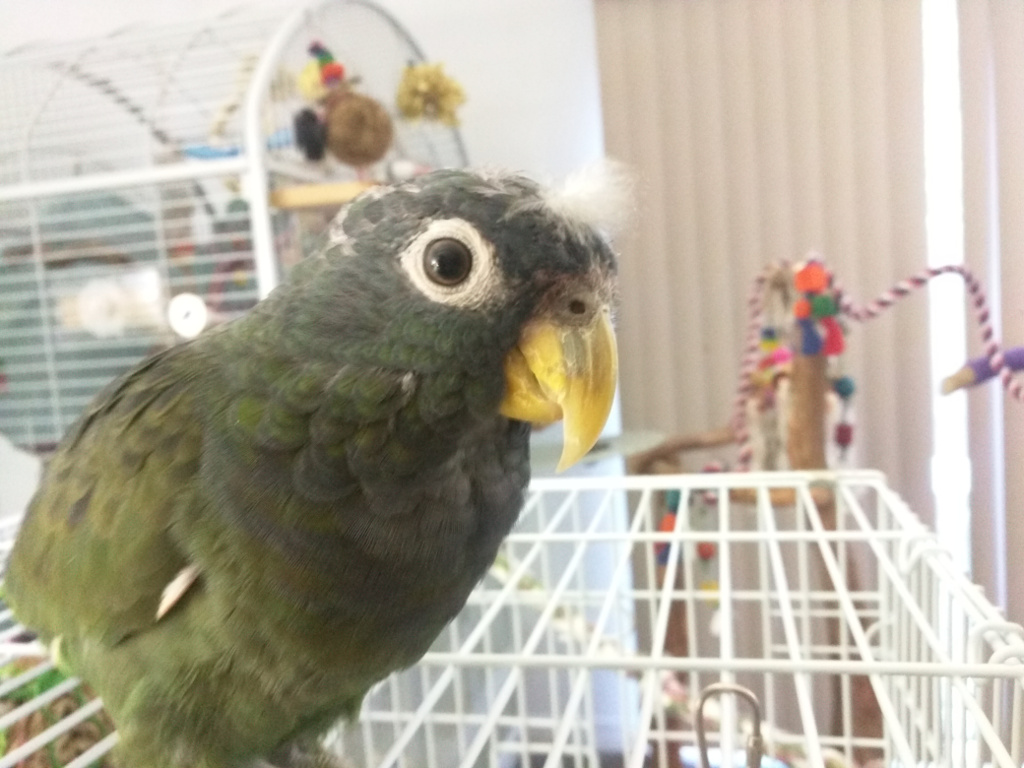
\includegraphics[scale=.15]{img/george}
        \caption{George}
      \end{figure}
    \end{column}
    \begin{column}{0.5\textwidth}
      \begin{figure}
        
\includegraphics[scale=.15]{img/george_blurry}
        \caption{Unfocused George}
      \end{figure}
    \end{column}
  \end{columns}
\end{frame}

\begin{frame}
  \frametitle{Image Convolution}

  Convolution is a common image processing technique that applies a
  \emph{kernel} to an image, resulting in effects such as blurring,
  sharpening, or edge detection.

  \begin{tiny}
    \begin{figure}[fragile]
      \[
        \begin{bmatrix}
          0.0625 & 0.125 & 0.0625 \\
          0.125 & 0.25 & 0.125 \\
          0.125 & 0.25 & 0.125
        \end{bmatrix} *
        \begin{bmatrix}
          0 & 1 & 2 & 1 & 0 \\
          1 & 1 & 2 & 1 & 1 \\
          1 & 2 & 2 & 2 & 1 \\
          1 & 1 & 2 & 1 & 1 \\
          0 & 1 & 2 & 1 & 0
        \end{bmatrix} =
        \begin{bmatrix}
          0.3125 & 0.8125  &  1.125   &  0.8125  &  0.3125 \\
          0.75   & 1.5625  &  2.0     &  1.5625  &  0.75   \\
          1.0625 & 1.8125  &  2.125   &  1.8125  &  1.0625 \\
          0.9375 & 1.75    &  2.125   &  1.75    &  0.9375 \\
          0.5    & 1.125   &  1.5     &  1.125   &  0.5
        \end{bmatrix}
      \]
      \caption{Application of the gaussian kernel}
    \end{figure}
  \end{tiny}
\end{frame}

\begin{frame}[fragile]
  Let's take another look at kernel application.  We'll step through
  and get an idea of what's happening:

  \frametitle{Image Convolution}
  \begin{figure}
    \animategraphics[loop,controls,width=0.6\linewidth]{2}{img/conv_anim-}{0}{8}
    \caption{Application of a kernel}
  \end{figure}
\end{frame}

\begin{frame}
  \frametitle{Example Code}

  Let's look at, and run, some code.
\end{frame}

\section{In Conclusion}

\begin{frame}
  \frametitle{TensorFlow is Useful Beyond ML}

  TensorFlow provides a framework for executing linear transformations
  on data without requiring that those operations be strictly tied to
  machine learning uses.  Many of the techniques are sufficiently
  general to be used in other situations as well.
\end{frame}

\begin{frame}
  \frametitle{TensorFlow is Fun}

  TensorFlow provides high-level abstractions that make it really
  trivial to do fun sample applications.  Digging into really
  complicated stuff is... harder, but by then you're already hooked!
\end{frame}

\subsection{Questions?}

\end{document}
